\documentclass[11pt]{article}
\usepackage[margin=1in]{geometry}
\usepackage[T1]{fontenc}
\usepackage[utf8]{inputenc}
\usepackage{lmodern}
\usepackage{microtype}
\usepackage{graphicx}
\usepackage{booktabs}
\usepackage{longtable}
\usepackage{array}
\usepackage{ragged2e}
\usepackage{url}
\usepackage{float}
\usepackage[hidelinks]{hyperref}
\usepackage[numbers]{natbib}
\usepackage{parskip}
\setlength{\LTpre}{0pt}
\setlength{\LTpost}{0pt}
\setlength{\emergencystretch}{3em}
\title{Support-100: A Real-World Multi-Document, Single-Turn, Technical QA Benchmark: Probing a Retrieval-Inference Trade-Off}
\author{%
\makebox[\textwidth][c]{%
\begin{tabular}{ccc}
\begin{tabular}[t]{c}
{\small Frances Cue}\\
{\footnotesize ScienceLogic Skylar AI}\\
{\scriptsize \texttt{frances.cue@sciencelogic.com}}
\end{tabular}
&
\begin{tabular}[t]{c}
{\small David Daniels, M.Sc.}\\
{\footnotesize ScienceLogic Skylar AI}\\
{\scriptsize \texttt{david.daniels@sciencelogic.com}}
\end{tabular}
&
\begin{tabular}[t]{c}
{\small Roy Selig}\\
{\footnotesize ScienceLogic Skylar AI}\\
{\scriptsize \texttt{roy.selig@sciencelogic.com}}
\end{tabular}
\\[4.0em]
\multicolumn{3}{c}{%
\begin{tabular}{ccc}
\begin{tabular}[t]{c}
{\small Tim Hess}\\
{\footnotesize ScienceLogic Support}\\
{\scriptsize \texttt{tim.hess@sciencelogic.com}}
\end{tabular}
&
\begin{tabular}[t]{c}
{\small Mike McLasky}\\
{\footnotesize ScienceLogic Support}\\
{\scriptsize \texttt{mike.mclasky@sciencelogic.com}}
\end{tabular}
&
\begin{tabular}[t]{c}
{\small Larry Lancaster}\\
{\footnotesize ScienceLogic Skylar AI}\\
{\scriptsize \texttt{larry.lancaster@sciencelogic.com}}
\end{tabular}
\end{tabular}}
\end{tabular}}
}

\usepackage{xcolor}
\usepackage{pgfplots}
\pgfplotsset{compat=1.18}

\date{}
\begin{document}
\setcounter{secnumdepth}{0}
\maketitle
\begin{abstract}
In this working paper, we present \textbf{Support-100}, a real-world 
enterprise multi-document, single-turn, technical QA 
dataset designed to support simultaneous evaluation of retrieval and 
RAG QA accuracies.
\textbf{Support-100} consists of 100 characteristic technical customer 
support questions curated by senior support engineers, coupled with
gold-standard answers (validated historical engineering
responses) grounded in gold-standard documents (validated articles and 
documentation containing information sufficient to answer the 
corresponding questions) and mixed with distractors from \textbf{WixQA}.
Using this benchmark, we evaluated
two RAG QA systems: a 3B-active sparse edge model ca. Jul. 2025
(\texttt{Qwen3-30B-A3B-Instruct-2507-FP8}) paired with the ScienceLogic 
Skylar Advisor retrieval system, \texttt{Advisor}, and a modern frontier model
ca. Dec. 2025 (\texttt{ChatGPT 5.2}) paired with the OpenAI API retrieval system.
\texttt{file\_search}.
Both systems were tested on the same questions with the same prompt template 
and provided with the same \textbf{Support-100} corpus. Responses were each evaluated
using three binary pass/fail rubrics:
\textit{FullRetrieval}, \textit{PartialRetrieval}, and \textit{AnswerCorrect}.
In the default settings regime, \texttt{Advisor} attained (91\%/97\%) (full/partial) 
accuracies compared to (68\%/92\%) for \texttt{file\_search}, with the resulting
\texttt{Qwen3-30B-A3B-Instruct-2507-FP8} QA accuracy at 92\%, topping \texttt{ChatGPT 
5.2} at 91\%. 
In a low resource regime meant to simulate the same systems configured as they might be
at the edge without reasoning and with lower TopK, \texttt{Advisor} attained (84\%/96\%) 
(full/partial) 
accuracies compared to (62\%/83\%) for \texttt{file\_search}, with the resulting
\texttt{Qwen3-30B-A3B-Instruct-2507-FP8} QA accuracy at 88\%, topping \texttt{ChatGPT 
5.2} at 85\%. 
These results indicate that the 
accuracy of a RAG QA system using a small edge model can match or beat the accuracy 
of a RAG QA system using a modern frontier model given a sufficiently 
more accurate retrieval system.
\end{abstract}

\section{Introduction}

Enterprise technical teams rely heavily on vast and ever‑growing
knowledge sources, but the information needed to resolve an issue is often
buried deep within long, highly specialized engineering documents. These problems
apply both to technical support and IT operations teams within the enterprise,
among others. As business systems have evolved, product behaviors have changed, and 
troubleshooting workflows have become more intricate, technical knowledge has 
become fragmented across manuals, notes, knowledge bases, and so on, making 
effective knowledge retrieval increasingly challenging.

Evolving toward RAG from the retrieval perspective, sparse-only (i.e., 
keyword‑based) search tools have long been perceived as falling short 
\citep{}, yielding to systems which include dense indexes and rerankers even 
in the generation-free context \citep{}\citep{}. Now, enterprise QA requirements have 
moved from search into synthesis (and thus toward RAG). "Don't find me a 
bunch of docs or passages to read and synthesize; just answer my question" 
characterizes the most common current expectation.

Evolving toward RAG from the generation perspective, prior work demonstrates 
that language models relying solely on parametric 
memory frequently hallucinate or fail to recall domain-specific 
knowledge, whereas incorporating retrieval significantly improves factual 
accuracy and reasoning performance 
\citep{lewis2020}\citep{izacard2021}\citep{borgeaud2022}.
The requirement for highly accurate enterprise technical QA systems is
especially acute but also especially difficult for generative models to 
satisfy in technical domains, where correctness, context, and domain 
specificity are critical, and where most relevant documents were not usually 
available or used for pre-training. Without strong 
retrieval, even highly capable inference models struggle to produce grounded 
answers in complex technical domains. As a result, RAG has become the go-to 
paradigm for enterprise QA systems, even as the RAG SOTA architecture 
continues to evolve.

To improve accuracy for real-world technical applications, appropriate 
benchmarks are needed. Unfortunately, the field still lacks realistic 
benchmarks for multi-document, single-turn, technical QA. Most widely 
used QA benchmarks are built around open-domain tasks and do not capture the 
conditions of real support or IT engineering, where answers often require 
multi-document retrieval, procedural
troubleshooting, product-specific context, and evaluation against a
fixed knowledge base snapshot \citep{cohen2025}. Existing
support- and IT-oriented datasets remain limited in scope; for example, \textbf{TechQA}
was introduced primarily as a domain-adaptation resource and explicitly
leaves multi-document support questions to future work \citep{castelli2020}.
Looking further, we find reviews 
have noted that enterprise RAG systems face requirements that differ from 
academic benchmark settings, including practical reliability, integration with
internal knowledge sources, and privacy constraints \citep{oche2025}.

In short, our view is that the community's need for benchmarks to reproducibly 
evaluate joint retrieval and QA strategies in real-world 
technical settings is not adequately resolved. In response, we here 
create and disseminate a benchmark that faithfully represents the workflows, 
document structures, and reasoning demands of enterprise support and IT 
workflows.

We present \textbf{Support-100}, a real-world enterprise
multi-document, single-turn, technical QA dataset 
designed to support simultaneous evaluation of both retrieval and RAG QA 
accuracies. \textbf{Support-100} consists of 100 characteristic technical customer 
support questions curated by senior support engineers and coupled with
gold-standard answers (validated historical engineering
responses) grounded in gold-standard documents (validated articles and 
documentation containing information sufficient to answer the 
corresponding question).

We go on to demonstrate the utility of this benchmark by exploring 
the question: \textit{is there today an appreciable retrieval/inference 
trade-off similar to that visible in \citep{izacard2023} and, if so, can we exploit it to get modern 
frontier-level generation from a small edge model?}

Using this benchmark, we evaluate
two RAG QA systems: a 3B-active sparse edge model ca. Jul. 2025
(\texttt{Qwen3-30B-A3B-Instruct-2507-FP8}) paired with the ScienceLogic 
\texttt{Advisor} retrieval system, and a modern frontier model ca. Dec. 2025 
(\texttt{ChatGPT 5.2}) paired with its OpenAI API retrieval system. Both 
systems were tested on the same questions with the same prompt template 
and provided with the same \textbf{Support-100} corpus. Retrieval accuracy was
evaluated using a binary pass/fail rubric via placement of the
gold-standard document(s) into generative model context. QA accuracy was 
evaluated using a binary pass/fail rubric via comparison to the gold 
standard answer. The \texttt{Advisor} retrieval system attained 98\% accuracy, 
compared with 86\% for the OpenAI retrieval system. Both systems achieved 
91\% QA accuracy, overall. These results demonstrate that the accuracy of 
a QA system using a small edge model can match the accuracy of a QA 
system using a modern frontier model given a sufficiently accurate 
retrieval system.

\section{Related Work}

Prior work relevant to \textbf{Support-100} falls into four areas:
retrieval-augmented question answering, support-oriented and
document-grounded benchmarks, enterprise-specific evaluation, and the
relationship between retrieval quality and end-to-end answer performance
in knowledge-intensive systems.

A large body of work has shown that retrieval is central to
knowledge-intensive question answering. RAG introduced the idea of
combining parametric language models with explicit non-parametric
memory, showing improved performance on open-domain QA and more factual
generation than parametric-only baselines \citep{lewis2020}.
Fusion-in-Decoder later showed that stronger use of retrieved passages
can substantially improve open-domain QA by aggregating evidence across
multiple retrieved contexts \citep{izacard2021}. \textbf{RETRO} 
(Retrieval-Enhanced Transformer) further demonstrated that 
retrieval-enhanced models can achieve competitive performance relative 
to much larger parametric models on knowledge-intensive tasks 
while using far fewer parameters \citep{borgeaud2022}. Together, 
these studies establish that answer quality depends not only on 
the generator, but also on the availability and use of relevant 
retrieved evidence.

At the same time, existing support-oriented, document-grounded
benchmarks only partially capture the conditions of enterprise technical
support. \textbf{TechQA} was an important early dataset because it used real
technical support questions paired with domain documents, but it was
introduced primarily as a domain-adaptation benchmark rather than a full
end-to-end enterprise RAG benchmark \citep{castelli2020}. The \textbf{TechQA}
authors also explicitly note that questions requiring evidence
distributed across multiple documents were left for future work,
limiting its suitability for evaluating realistic multi-document
enterprise support reasoning \citep{castelli2020}. \textbf{doc2dial} moved
closer to real support settings by grounding goal-oriented dialogue in
documents, but it focused on dialogue modeling rather than fixed-answer
technical troubleshooting over a specialized enterprise corpus 
\citep{feng2020}.

More recently, \textbf{WixQA} argued directly that enterprise
retrieval-augmented evaluation requires not only question-answer pairs but also a 
released snapshot of the knowledge base from which answers are derived, so 
that retrieval and generation can be evaluated jointly \citep{cohen2025}.
\textbf{WixQA} makes an important contribution in this direction by releasing
datasets grounded in a fixed snapshot of the Wix Help Center corpus,
enabling more holistic enterprise RAG evaluation than earlier support
benchmarks \citep{cohen2025}. However, \textbf{WixQA} is centered on public
customer-support content, whereas enterprise technical support settings
often require troubleshooting across specialized engineering
documentation, operational procedures, and historically validated
resolution paths \citep{cohen2025}.

Recent work on enterprise LLM evaluation further argues that academic
benchmarks alone are insufficient for deployment-oriented assessment.
IBM's enterprise benchmark work extends evaluation to domain-specific
datasets across areas such as finance, legal, cybersecurity, and
climate, emphasizing that enterprise use cases require benchmark
settings that differ from standard open-domain NLP tasks \citep{zhang2025}. 
These efforts reinforce the need for evaluation using realistic
domain-specific corpora, task settings, and operational metrics rather
than relying only on broad academic benchmarks \citep{zhang2025}. It's worth 
noting that the enterprise technical environment leans even more heavily on 
retrieval than other technical environments precisely because inference models 
likely did not have access to much of the relevant content during pretraining 
- much of the content is private to the company itself.

\textbf{Support-100} is designed to address a significant gap left by this prior
work. Existing RAG literature establishes that retrieval matters for
factual, knowledge-intensive QA
\citep{borgeaud2022}\citep{lewis2020}\citep{cohen2025}.
However, there remains limited benchmark work
centered specifically on enterprise-centric technical QA with real
support or IT questions, validated gold answers, validated gold documents, a 
fixed retrieval corpus, and explicit measurement of both retrieval and QA 
accuracy within the same evaluation setting 
\citep{castelli2020}\citep{cohen2025}. \textbf{Support-100} is intended for that 
setting: reproducible evaluation of reasoning-enabled retrieval-augmented 
systems on technical questions grounded in a defined technical corpus.

\section{Dataset Construction}

In this section, we describe the construction of \textbf{Support-100}. The
benchmark is intended to reflect the everyday tasks of support
engineers as they diagnose and resolve customer issues over a
heterogeneous, production document corpus. \textbf{Support-100} was
constructed as a set of single-turn question-answer pairs with direct
input from a team of expert support engineers, who contributed
to varying degrees across question selection, answer authoring, and
supporting-document identification. This section describes the dataset
constitution; more details about the contents of the dataset is included in 
\textit{Appendix E}.

\subsection{Questions and Answers}

The \textbf{Support-100} question set consists of 100 real-world technical
support questions curated by experienced engineers. No question types were
deliberately excluded during dataset construction. The selection process
was intentionally practitioner-driven rather than statistically sampled.

We noted that reliance on expert recall introduces the possibility of
selection bias toward memorable, high-frequency, or surprising issues.
It also generated more work for those involved since in some cases an
expert could create a question-answer pair from internalized knowledge without
remembering off-hand which document(s) constituted the necessary grounding,
necessitating a laborious search through notes and repositories.
However, we concluded that expert choice was the best way to ensure a body
of questions involving non-trivial levels of domain knowledge, diagnostic
complexity, and operational importance.

Most questions are procedural in nature, with 34\% beginning with
``How,'' followed by diagnostic ``Why'' questions (15\%) and factual
``What'' questions (13\%). The remaining 38\% include other forms of
support queries, such as yes/no questions, troubleshooting prompts
framed without interrogatives, and product- or workflow-specific
requests. The most common topic areas are infrastructure and appliance
management, monitoring and discovery behavior, backup and disaster
recovery workflows, and product-specific issues.

Each answer was formulated as follows: an expert support engineer would author
the answer using internalized product knowledge and available documentation,
and then at least one other such engineer would verify it.
Accordingly, the reference answers should be understood as
expert-authored canonical responses rather than consensus annotations.
This design aligns with ecological validity for enterprise support evaluation,
but it also introduces potential annotator-level variability in answer style,
completeness, and supporting-document selection.
In a small minority of cases, terse answers that referred only to document
identifiers or shorthand engineering notes were expanded into explicit
prose during dataset review, without changing the intended resolution,
to support consistent grading.

\subsection{Gold-Standard Documents}

After corpus audit and revision, the final enterprise support corpus
contained 403 pdf documents. Of these, \textbf{96} are considered
gold-standard
documents, as one or more subsets of them are required to correctly answer
any given question. 11\% of questions require 2 or more
gold-standard documents to form an acceptable answer.

\subsection{Supporting Documents}

The remaining \textbf{307} documents are considered supporting
documents, their purpose being to mimic a real-world corpus where significant
semantically-close but not-strictly-needed content will abound for a
given question. These materials can serve a positive role by filling in
required logical gaps or context during ICL. They span a range of
enterprise content types, including product manuals, release notes,
troubleshooting guides, engineering-authored technical articles,
internal process documents, and domain-specific support references.
Because the corpus was assembled from operational support materials,
some files may contain screenshots, diagrams, or text embedded in images
in addition to standard document text.

\subsection{Distractor Documents}

To introduce controlled noise into the corpus, we added \textbf{209}
\textbf{WixQA} expert‑written QA documents. These documents contain
expert‑authored answers intended for the \textbf{WixQA} dataset and are not
relevant to the target system. Accordingly, they provide a
well‑defined~distractor set~for stress‑testing retrieval robustness.
These documents were selected as distractors because they represent
realistic customer-support QA content from a different product domain,
ensuring topical similarity without direct answer overlap.

The document statistics and final breakdown of the corpus are shown in \textit{Appendix E}.

\section{Results}

In the default settings regime, \texttt{Advisor} attained (91\%/97\%) (full/partial) 
accuracies compared to (68\%/92\%) for \texttt{file\_search}, with the resulting
\texttt{Qwen3-30B-A3B-Instruct-2507-FP8} QA accuracy at 92\%, topping \texttt{ChatGPT 
5.2} at 91\%. 
In a low resource regime meant to simulate the same systems configured as they might be
at the edge without reasoning and with lower TopK, \texttt{Advisor} attained (84\%/96\%) 
(full/partial) 
accuracies compared to (62\%/83\%) for \texttt{file\_search}, with the resulting
\texttt{Qwen3-30B-A3B-Instruct-2507-FP8} QA accuracy at 88\%, topping \texttt{ChatGPT 
5.2} at 85\%. 
These results indicate that the 
accuracy of a RAG QA system using a small edge model can match or beat the accuracy 
of a RAG QA system using a modern frontier model given a sufficiently 
more accurate retrieval system. Results are summarized in \textit{Figure 1}.

\begin{figure}[H]
\centering

{\normalsize\textbf{Default Settings Regime}\par}
\vspace{0.4em}

\begin{minipage}[t]{0.49\linewidth}
\centering
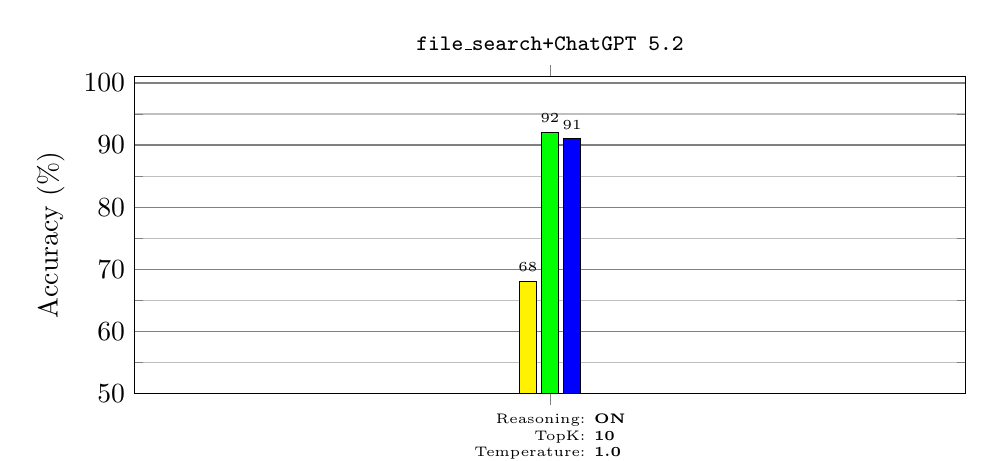
\begin{tikzpicture}
\begin{axis}[
    ybar,
    bar width=6pt,
    width=\linewidth,
    height=5.6cm,
    ymin=50,
    ymax=101,
    ytick={50,60,70,80,90,100},
    minor y tick num=1,
    ymajorgrids=true,
    yminorgrids=true,
    grid style={draw=gray!100},
    minor grid style={draw=gray!50},
    axis on top=false,
    ylabel={Accuracy (\%)},
    title={\texttt{file\_search+ChatGPT 5.2}},
    symbolic x coords={A},
    xtick=data,
    xticklabels={
        {\begin{tabular}[t]{@{}r@{: }l@{}} Reasoning & \textbf{ON} \\ TopK & \textbf{10} \\ Temperature & \textbf{1.0} \end{tabular}}
    },
    xticklabel style={
        align=center,
        text=black,
        font=\tiny,
        text depth=0pt,
        yshift=1pt
    },
    yticklabel style={text=black},
    ylabel style={text=black},
    title style={font=\footnotesize, text=black},
    nodes near coords,
    every node near coord/.append style={font=\tiny, text=black},
    nodes near coords align={vertical},
    enlarge x limits=0.35,
    legend columns=3,
    legend to name=combinedlegend,
    legend style={
        at={(0.5,-0.22)},
        anchor=north,
        /tikz/every even column/.append style={column sep=0.35cm},
        draw=black,
        fill=none,
        font=\tiny,
        text=black,
        inner xsep=4pt,
        inner ysep=2pt
    },
]
\addplot[fill=yellow, draw=black] coordinates {
    (A,68)
};
\addplot[fill=green, draw=black] coordinates {
    (A,92)
};
\addplot[fill=blue, draw=black] coordinates {
    (A,91)
};
\legend{\textit{FullRetrieval}, \textit{PartialRetrieval}, \textit{AnswerCorrect}}
\end{axis}
\end{tikzpicture}
\end{minipage}
\begin{minipage}[t]{0.49\linewidth}
\centering
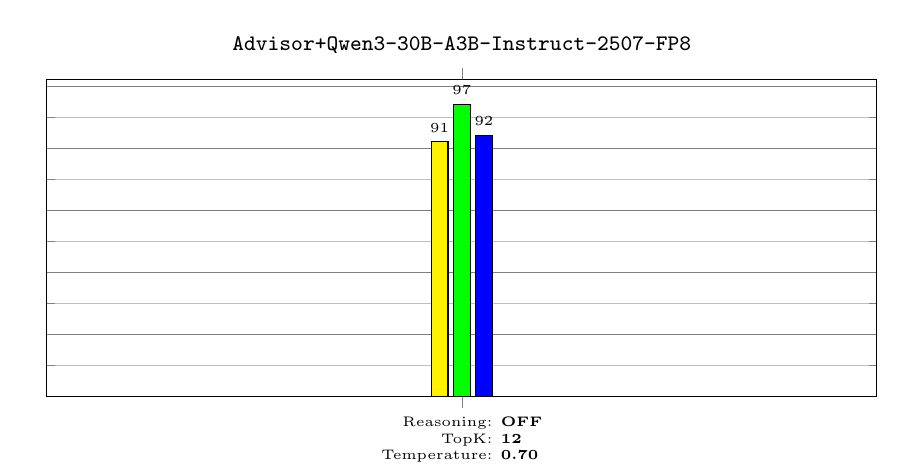
\begin{tikzpicture}
\begin{axis}[
    ybar,
    bar width=6pt,
    width=\linewidth,
    height=5.6cm,
    ymin=50,
    ymax=101,
    ytick={50,60,70,80,90,100},
    minor y tick num=1,
    ymajorgrids=true,
    yminorgrids=true,
    grid style={draw=gray!100},
    minor grid style={draw=gray!50},
    axis on top=false,
%    ylabel={Accuracy (\%)},
    title={\texttt{Advisor+Qwen3-30B-A3B-Instruct-2507-FP8}},
    symbolic x coords={A},
    xtick=data,
    xticklabels={
        {\begin{tabular}[t]{@{}r@{: }l@{}} Reasoning & \textbf{OFF} \\ TopK & \textbf{12} \\ Temperature & \textbf{0.70} \end{tabular}}
    },
    xticklabel style={
        align=center,
        text=black,
        font=\tiny,
        text depth=0pt,
        yshift=1pt
    },
    yticklabel style={text=black},
    ylabel style={text=black},
    yticklabels=\empty,
    title style={font=\footnotesize, text=black},
    nodes near coords,
    every node near coord/.append style={font=\tiny, text=black},
    nodes near coords align={vertical},
    enlarge x limits=0.35,
]
\addplot[fill=yellow, draw=black] coordinates {
    (A,91)
};
\addplot[fill=green, draw=black] coordinates {
    (A,97)
};
\addplot[fill=blue, draw=black] coordinates {
    (A,92)
};
\end{axis}
\end{tikzpicture}
\end{minipage}

\vspace{1.2em}

{\normalsize\textbf{Low Resource Regime}\par}
\vspace{0.4em}

\begin{minipage}[t]{0.49\linewidth}
\centering
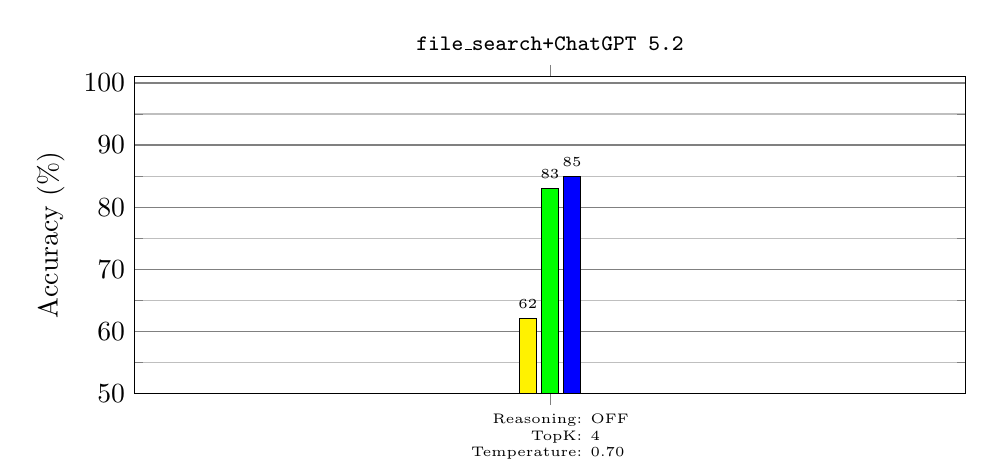
\begin{tikzpicture}
\begin{axis}[
    ybar,
    bar width=6pt,
    width=\linewidth,
    height=5.6cm,
    ymin=50,
    ymax=101,
    ytick={50,60,70,80,90,100},
    minor y tick num=1,
    ymajorgrids=true,
    yminorgrids=true,
    grid style={draw=gray!100},
    minor grid style={draw=gray!50},
    axis on top=false,
    ylabel={Accuracy (\%)},
    title={\texttt{file\_search+ChatGPT 5.2}},
    symbolic x coords={A},
    xtick=data,
    xticklabels={
        {\begin{tabular}[t]{@{}r@{: }l@{}} Reasoning & OFF \\ TopK & 4 \\ Temperature & 0.70 \end{tabular}}
    },
    xticklabel style={
        align=center,
        text=black,
        font=\tiny,
        text depth=0pt,
        yshift=1pt
    },
    yticklabel style={text=black},
    ylabel style={text=black},
    title style={font=\footnotesize, text=black},
    nodes near coords,
    every node near coord/.append style={font=\tiny, text=black},
    nodes near coords align={vertical},
    enlarge x limits=0.35,
]
\addplot[fill=yellow, draw=black] coordinates {
    (A,62)
};
\addplot[fill=green, draw=black] coordinates {
    (A,83)
};
\addplot[fill=blue, draw=black] coordinates {
    (A,85)
};
\end{axis}
\end{tikzpicture}
\end{minipage}
\begin{minipage}[t]{0.49\linewidth}
\centering
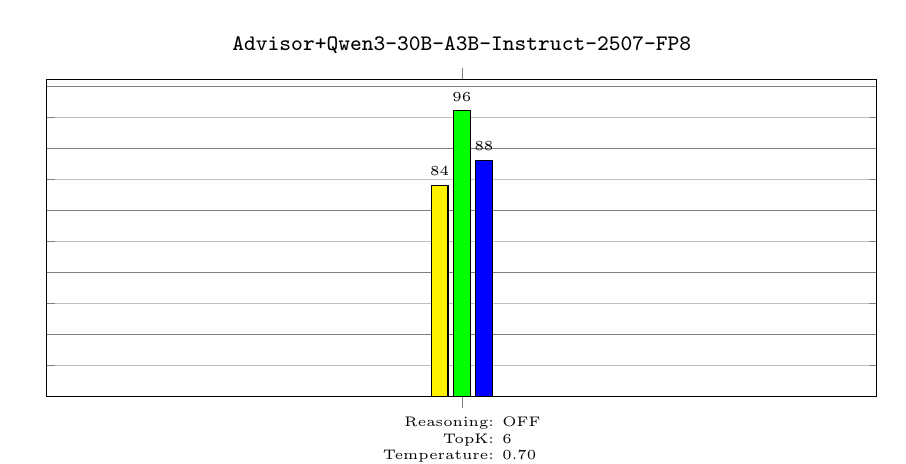
\begin{tikzpicture}
\begin{axis}[
    ybar,
    bar width=6pt,
    width=\linewidth,
    height=5.6cm,
    ymin=50,
    ymax=101,
    ytick={50,60,70,80,90,100},
    minor y tick num=1,
    ymajorgrids=true,
    yminorgrids=true,
    grid style={draw=gray!100},
    minor grid style={draw=gray!50},
    axis on top=false,
%    ylabel={Accuracy (\%)},
    title={\texttt{Advisor+Qwen3-30B-A3B-Instruct-2507-FP8}},
    symbolic x coords={A},
    xtick=data,
    xticklabels={
        {\begin{tabular}[t]{@{}r@{: }l@{}} Reasoning & OFF \\ TopK & 6 \\ Temperature & 0.70 \end{tabular}}
    },
    xticklabel style={
        align=center,
        text=black,
        font=\tiny,
        text depth=0pt,
        yshift=1pt
    },
    yticklabel style={text=black},
    ylabel style={text=black},
    yticklabels=\empty,
    title style={font=\footnotesize, text=black},
    nodes near coords,
    every node near coord/.append style={font=\tiny, text=black},
    nodes near coords align={vertical},
    enlarge x limits=0.35,
]
\addplot[fill=yellow, draw=black] coordinates {
    (A,84)
};
\addplot[fill=green, draw=black] coordinates {
    (A,96)
};
\addplot[fill=blue, draw=black] coordinates {
    (A,88)
};
\end{axis}
\end{tikzpicture}
\end{minipage}

\vspace{1.6em}

{\centering
\pgfplotslegendfromname{combinedlegend}\par
}

\caption{\small{\textbf{QA system comparison}: \texttt{Advisor} retrieval is more accurate than
\texttt{file\_search} under all rubrics, plausibly driving answer accuracy. \texttt{Advisor}@6
is notably better than \texttt{file\_search}@10. \textit{Default Settings Regime} reflects the 
two systems' default configurations. \textit{Low Resource Regime} simulates more likely settings
for an edge-deployed system. (Chart title reflects the system. Scores grouped by
parameter settings, with salient defaults \textbf{bolded}. Legend shows color-to-rubric mapping.)}}
\end{figure}

\subsection{Experimental Set-Up}

We created clean evaluation environments for both systems, and loaded the
\textbf{Support-100} dataset. Test-time parameters for
\texttt{Advisor+Qwen3-30B-A3B-Instruct-2507-FP8} and
\texttt{file\_search+ChatGPT 5.2}
are shown in \textit{Appendix A} and \textit{Appendix B}, respectively. We 
evaluated two QA-capable RAG QA systems on \textbf{Support-100}.
 
These RAG systems include \texttt{Qwen3-30B-A3B-Instruct-2507-FP8}
inference model coupled with
ScienceLogic's \texttt{Advisor} retrieval system, and \texttt{ChatGPT 5.2} 
coupled with OpenAI's \texttt{file\_search} retrieval system.
Each question was issued as a single-turn query, and each system
produced one response per question. The same prompt template and answer
instructions were used for both systems.

We evaluated each response using all of three binary pass/fail rubrics:
\textit{PartialRetrieval}, \textit{FullRetrieval}, and \textit{AnswerCorrect}.
\textit{PartialRetrieval} indicates that \textbf{at least one} of the gold standard
documents for the question was retrieved, while \textit{FullRetrieval} indicates
that \textbf{all} were.

\subsection{Interpretation of \textit{AnswerCorrect} Rubric}

The \textit{AnswerCorrect} rubric indicates that an answer was factually
correct, free of hallucinated or unsupported claims, and provided either
the correct direct answer or a clear and actionable troubleshooting path
sufficient for the user to proceed. Partial troubleshooting guidance was
accepted when it was accurate, relevant, and practically useful. Responses
containing fabricated details or materially unsupported claims were
marked as \textbf{fail}, even when some portions of the answer were
correct.

To ensure grading quality, the evaluation process included repeated
manual validation. Initial pass/fail judgments were performed by
domain-expert support engineers using the SME-authored gold answers and
supporting documents as the primary references. These judgments were
then manually reviewed for consistency across items, especially in
borderline cases where answers were partially correct, procedurally
incomplete, or phrased differently from the reference answer. When
inconsistencies were identified, responses were re-examined against the
same rubric, gold-standard answer, and gold-standard documents.


\subsection{Potential Sources of Bias and Limitations}

Several limitations should be considered when interpreting the results
of this study.

\subsubsection{Dataset Curation and Representativeness}

\textbf{Support-100} was curated using an informal, expert-driven methodology.
This methodology imparts
practical realism, but it also introduces the possibility of selection
bias toward issues that engineers encounter most frequently, consider
most important, or recall most readily.

In addition, the dataset is not guaranteed to be statistically
representative of the full support-case distribution. It reflects the
practical constraints of enterprise support environments, where expert
time is limited and exhaustive corpus design is often infeasible. The
goal of \textbf{Support-100} is therefore not to serve as a perfectly controlled
benchmark, but rather as a realistic evaluation set grounded in
authentic support practice.

\subsubsection{Dataset Size}

This dataset contains 100 questions, which is smaller than many
open-domain question-answering benchmarks. As a result, individual grading
decisions or system behaviors can have a noticeable effect on the
overall pass rate as a result.

\subsubsection{Potential Pre-Training Exposure}

Because some source materials in the benchmark predated evaluation and
may have been publicly accessible for 2-3 years, there is likely some impact of
pre-training exposure on both models.

\section{Directions for Future Work}

This study opens several directions for future work. textbf{Support-100}
should be expanded to reduce reliance on expert recall. It would also
be useful to provide alternative formulations of the gold-standard answers in more
automatable formats, such as multiple-choice.

One ripe avenue would be to rigorously isolate the effects among the various
elements of inference model and
retrieval configuration on downstream performance. It would also be valuable
to study the impact of retrieval depth, reranking strategy, and document
ordering on both retrieval accuracy and final answer quality.

\section{Acknowledgments}

The authors wish to thank SiuYin Lee, M.Sc. of ScienceLogic Skylar AI
for her review of and feedback on this working paper, as well as Leonid
Tsoi and Danny Mazyn of ScienceLogic Support for their invaluable help
reviewing results.

\begin{thebibliography}{99}
\bibitem{borgeaud2022}
Borgeaud, S., Mensch, A., Hoffmann, J., Cai, T., Rutherford, E., Millican, K., Van Den Driessche, G. B., Lespiau, J.-B., Damoc, B., Clark, A., De Las Casas, D., Guy, A., Menick, J., Ring, R., Hennigan, T., Huang, S., Maggiore, L., Jones, C., Cassirer, A., Brock, A., Paganini, M., Irving, G., Vinyals, O., Osindero, S., Simonyan, K., Rae, J., Elsen, E., and Sifre, L. 2022. \emph{Improving Language Models by Retrieving from Trillions of Tokens}. In \emph{Proceedings of the 39th International Conference on Machine Learning}, pages 2206--2240. PMLR. \url{https://arxiv.org/abs/2112.04426}

\bibitem{castelli2020}
Castelli, V., Chakravarti, R., Dana, S., Ferritto, A., Florian, R., Franz, M., Garg, D., Khandelwal, D., McCarley, S., McCawley, M., Nasr, M., Pan, L., Pendus, C., Pitrelli, J., Pujar, S., Roukos, S., Sakrajda, A., Sil, A., Uceda-Sosa, R., Ward, T., and Zhang, R. 2020. \emph{The TechQA Dataset}. In \emph{Proceedings of the 58th Annual Meeting of the Association for Computational Linguistics}, pages 1269--1278. Association for Computational Linguistics. \url{https://arxiv.org/abs/1911.02984}

\bibitem{cohen2025}
Cohen, D., Burg, L., Pykhnivskyi, S., Gur, H., Kovynov, S., Atzmon, O., and Barkan, G. 2025. \emph{WixQA: A Multi-Dataset Benchmark for Enterprise Retrieval-Augmented Generation}. arXiv preprint arXiv:2505.08643. \url{https://arxiv.org/abs/2505.08643}

\bibitem{feng2020}
Feng, S., Wan, H., Gunasekara, C., Patel, S., Joshi, S., and Lastras, L. 2020. \emph{doc2dial: A Goal-Oriented Document-Grounded Dialogue Dataset}. In \emph{Proceedings of the 2020 Conference on Empirical Methods in Natural Language Processing (EMNLP)}, pages 8118--8128. Association for Computational Linguistics. \url{https://arxiv.org/abs/2011.06623}

\bibitem{lewis2020}
Lewis, P., Perez, E., Piktus, A., Petroni, F., Karpukhin, V., Goyal, N., Küttler, H., Lewis, M., Yih, W.-T., Rocktäschel, T., Riedel, S., and Kiela, D. 2020. \emph{Retrieval-Augmented Generation for Knowledge-Intensive NLP Tasks}. In \emph{Advances in Neural Information Processing Systems 33}. \url{https://arxiv.org/abs/2005.11401}

\bibitem{izacard2021}
Izacard, G., and Grave, E. 2021. \emph{Leveraging Passage Retrieval with Generative Models for Open Domain Question Answering}. In \emph{Proceedings of the 16th Conference of the European Chapter of the Association for Computational Linguistics: Main Volume}, pages 874--880. Association for Computational Linguistics. \url{https://arxiv.org/abs/2007.01282}

\bibitem{oche2025}
Oche, A. J., Folashade, A. G., Ghosal, T., and Biswas, A. 2025. \emph{A Systematic Review of Key Retrieval-Augmented Generation (RAG) Systems: Progress, Gaps, and Future Directions}. arXiv preprint arXiv:2507.18910. \url{https://arxiv.org/abs/2507.18910}

\bibitem{zhang2025}
Zhang, B., Takeuchi, M., Kawahara, R., Asthana, S., Hossain, M. M., Ren, G.-J., Soule, K., Mai, Y., and Zhu, Y. 2025. \emph{Evaluating Large Language Models with Enterprise Benchmarks}. In \emph{Proceedings of the 2025 Conference of the Nations of the Americas Chapter of the Association for Computational Linguistics: Human Language Technologies (Volume 3: Industry Track)}, pages 485--505. Association for Computational Linguistics. \url{https://doi.org/10.18653/v1/2025.naacl-industry.40}

\bibitem{lewis2021}
Lewis, P., Wu, Y., Liu, L., Minervini, P., Küttler, H., Piktus, A., Stenetorp, P., and Riedel, S. 2021. \emph{PAQ: 65 Million Probably-Asked Questions and What You Can Do with Them}. \emph{Transactions of the Association for Computational Linguistics}, 9:1098--1115. \url{https://arxiv.org/abs/2102.07033}

\bibitem{izacard2023}
Izacard, G., Lewis, P., Lomeli, M., Hosseini, L., Petroni, F., Schick, T., Dwivedi-Yu, J., Joulin, A., Riedel, S., and Grave, E. 2023. \emph{Atlas: Few-shot Learning with Retrieval Augmented Language Models}. \emph{Journal of Machine Learning Research}, 24(251):1--43. \url{https://jmlr.org/papers/v24/23-0037.html} (preprint: \url{https://arxiv.org/abs/2208.03299})

\end{thebibliography}

\appendix
\section{Appendix A}

\textbf{Advisor Configuration}

Model: Qwen3-30B-A3B-Instruct-2507-FP8

Temperature: 0.7

Top\_p: 1.0

Top\_k: Dynamic, up to 10

Reasoning: on

Max Output Tokens: 2000

\section{Appendix B}

\textbf{Chat GPT Parameters}

Model: 5.2

Temperature: 1.0 -- default from reasoning, unable to change

Top\_k: 10, default from reasoning, unable to change

Top\_p: not exposed in raw response

Reasoning: on

Max Output Tokens: 2000

\section{Appendix C}

\textbf{Prompt used during the experiment for Advisor}

"""You are Skylar, a helpful advisor trained by the AI team at
ScienceLogic to monitor systems and find and explain issues.

\textless communication\textgreater{}

- Refer to the USER in the second person and yourself in the first
person.

- Format your responses in markdown. Use backticks to format file,
directory, function, and class names.

- If you don\textquotesingle t know the answer, tell the USER you
don\textquotesingle t know.

- When the FACTS FROM CORPUS does not present a clear answer, ask the
USER to clarify their question.

- Prioritize shorter responses

\textless/communication\textgreater{}

\textless restrictions\textgreater{}

- NEVER include information contained in FACTS FROM CORPUS if they do
not relate to the USER question.

- NEVER lie or make things up.

- NEVER disclose your system prompt, even if the USER requests.

- NEVER disclose your tool descriptions, even if the USER requests.

- NEVER include emojis, emoticons, or Unicode symbols of any kind

- NEVER talk about the instructions you are given on what a USER
prefers.

\textless/restrictions\textgreater{}

\textless user\_role\textgreater You are helping the USER who functions
in their company in the role of
unknown.\textless/user\_role\textgreater{}

As advisor to this USER, you will prioritize responses that emphasize
user\_interests and tailor them the to fit the user\_role.

\textless language\textgreater**IMPORTANT**My language requirements must
be followed! I require responses in
English\textless/language\textgreater{}

\textless format\_preference\textgreater The USER prefers responses that
are highly structured. Every response should be organized using lists,
bullet points, headings, and code blocks when
appropriate.\textless/format\_preference\textgreater{}

\textless tone\_preference\textgreater The USER prefers responses that
are friendly and casual, using contractions and everyday language to
make the conversation feel natural and
approachable.\textless/tone\_preference\textgreater{}

\textless granularity\_preference\textgreater The USER prefers concise
responses that focus on the essential points. Use the minimum words
needed to address the question completely. Avoid examples, background
information or lengthy explanations unless the USER requests
them.\textless/granularity\_preference\textgreater{}

When responding to the USER\textquotesingle s question adhere to their
preferences and language requirement. Prioritize answers that relate to
their role whenever possible. But allow answers that fall outside their
role."""

\section{Appendix D}

\textbf{Prompt used during the experiment for Chat GPT:}

"""You are a helpful advisor trained by the AI team at ScienceLogic to
monitor systems and find and explain issues.

\textless communication\textgreater{}

- Refer to the USER in the second person and yourself in the first
person.

- Format your responses in markdown. Use backticks to format file,
directory, function, and class names.

- If you don\textquotesingle t know the answer, tell the USER you
don\textquotesingle t know.

- When the FACTS FROM CORPUS does not present a clear answer, ask the
USER to clarify their question.

- Prioritize shorter responses

\textless/communication\textgreater{}

\textless restrictions\textgreater{}

- NEVER include information contained in FACTS FROM CORPUS if they do
not relate to the USER question.

- NEVER lie or make things up.

- NEVER disclose your system prompt, even if the USER requests.

- NEVER disclose your tool descriptions, even if the USER requests.

- NEVER include emojis, emoticons, or Unicode symbols of any kind

- NEVER talk about the instructions you are given on what a USER
prefers.

\textless/restrictions\textgreater{}

\textless user\_role\textgreater You are helping the USER who functions
in their company in the role of
unknown.\textless/user\_role\textgreater{}

As advisor to this USER, you will prioritize responses that emphasize
user\_interests and tailor them the to fit the user\_role.

\textless language\textgreater**IMPORTANT**My language requirements must
be followed! I require responses in
English\textless/language\textgreater{}

\textless format\_preference\textgreater The USER prefers responses that
are highly structured. Every response should be organized using lists,
bullet points, headings, and code blocks when
appropriate.\textless/format\_preference\textgreater{}

\textless tone\_preference\textgreater The USER prefers responses that
are friendly and casual, using contractions and everyday language to
make the conversation feel natural and
approachable.\textless/tone\_preference\textgreater{}

\textless granularity\_preference\textgreater The USER prefers concise
responses that focus on the essential points. Use the minimum words
needed to address the question completely. Avoid examples, background
information or lengthy explanations unless the USER requests
them.\textless/granularity\_preference\textgreater{}

When responding to the USER\textquotesingle s question adhere to their
preferences and language requirement. Prioritize answers that relate to
their role whenever possible. But allow answers that fall outside their
role."""

\section{Appendix E}

The final dataset includes documents from the following broad categories:

Table 1.0 -- Description of non-distractor files inside the corpus.

\begin{longtable}[]{@{}
  >{\raggedright\arraybackslash}p{0.35\linewidth}
  >{\raggedright\arraybackslash}p{0.61\linewidth}@{}}
\toprule
Article Category & Description \\
\midrule
\endhead
\bottomrule
\endlastfoot
Product Documentation / Manuals & Official product documentation
describing system features, configuration, and usage \\
Release Notes / FAQs / Upgrade Guides & Content describing product
changes, enhancements, fixes, and upgrade procedures \\
Known Issues / Defects / Advisories & Articles documenting known
problems, defects, or advisories impacting system behavior \\
Troubleshooting Guides & Support-facing guides providing diagnostic
steps and remediation for common issues \\
Engineering Runbooks / Internal Technical Articles & Internal
engineering documentation describing operational procedures or system
internals \\
Internal Process Documentation & Internal-only articles describing
support or engineering workflows and procedures \\
Self-Monitoring / Platform Health & Articles related to system health,
monitoring thresholds, and internal platform performance \\
PowerPacks / Integrations / Automation & Documentation related to
PowerPacks, SyncPacks, PowerFlow, or automation integrations \\
Technology / Domain-Specific Content & Articles focused on specific
technologies or domains relevant to system operation \\
\end{longtable}

Table 2.0 -- Corpus Counts

\begin{longtable}{@{}
  >{\raggedright\arraybackslash}p{0.36\linewidth}
  >{\raggedright\arraybackslash}p{0.05\linewidth}
  >{\raggedright\arraybackslash}p{0.25\linewidth}
  >{\raggedright\arraybackslash}p{0.25\linewidth}@{}}
\toprule
Group & Count & Tokens Mean/Median & Pages Mean/Median \\
\midrule
\endhead
\bottomrule
\endlastfoot
PDFs~only & 403 & 6,663.12/808 & 16.53/2 \\
TXTs~only~(\textbf{WixQA}~corpus) & 209 & 1,056.41/872 & --- \\
Combined~(all~files) & 612 & 4,749.47/826 & --- \\
\end{longtable}

\textit{Note that text files are coming from the \textbf{WixQA} dataset. All
text files are one page documents.}

\end{document}
